\documentclass{article}
\usepackage{indentfirst}
\usepackage{hyperref}
\hypersetup{
	colorlinks=true,
	urlcolor=blue,
	pdftitle={How to Set Up Your User Settings GUI Development Environment},
}
\usepackage{graphicx}
\graphicspath{ {./images/} }

\begin{document}
\begin{center}
\Large{How to Set Up Your User Settings GUI Development Environment}
\end{center}

\textbf{NOTE:} This guide is for setting up IntelliJ to work on the GUI code, if you are just using the device, or plan on only customizing the hardware, you won't need to follow these instructions.

\begin{enumerate}
  \item Install a JDK/SDK 17 (must be 17). This can be installed \href{https://www.oracle.com/java/technologies/downloads/}{here.} The basic settings can be used.
  \item Install the community version of InteeliJ \href{https://www.jetbrains.com/idea/download/}{here.}
  \begin{itemize}
    \item When you get to the Installation Options page on the wizard that has the option to "Update PATH variable (restart needed)" make sure to check the "Add "bin" folder to the PATH" box.
  \end{itemize}
  \item Create a new project, and on the side select it as a JavaFX project. Make sure the proper JDK is selected, then hit 'Next.'
    \begin{center}
    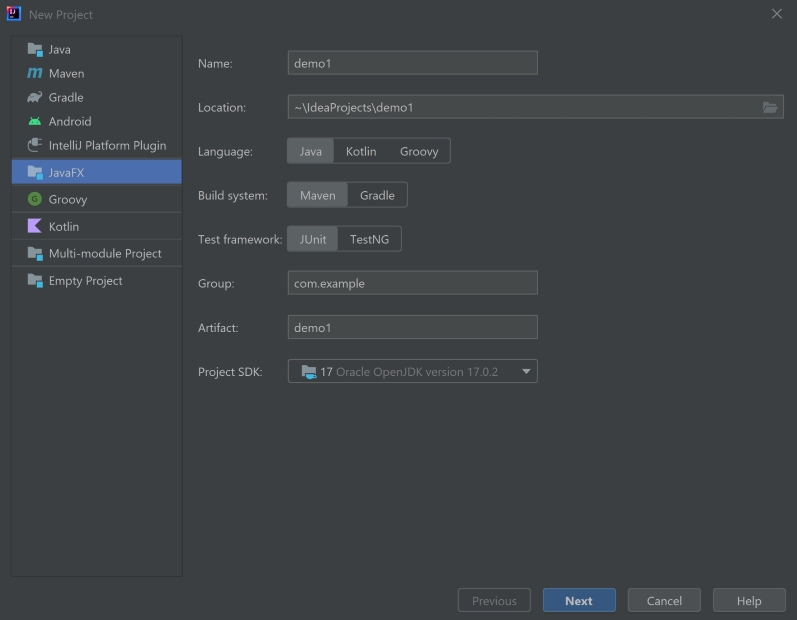
\includegraphics{DevGuideNewProject}
    \end{center}
\newpage
  \item Don't select any dependencies, and hit 'Finish.'
    \begin{center}
    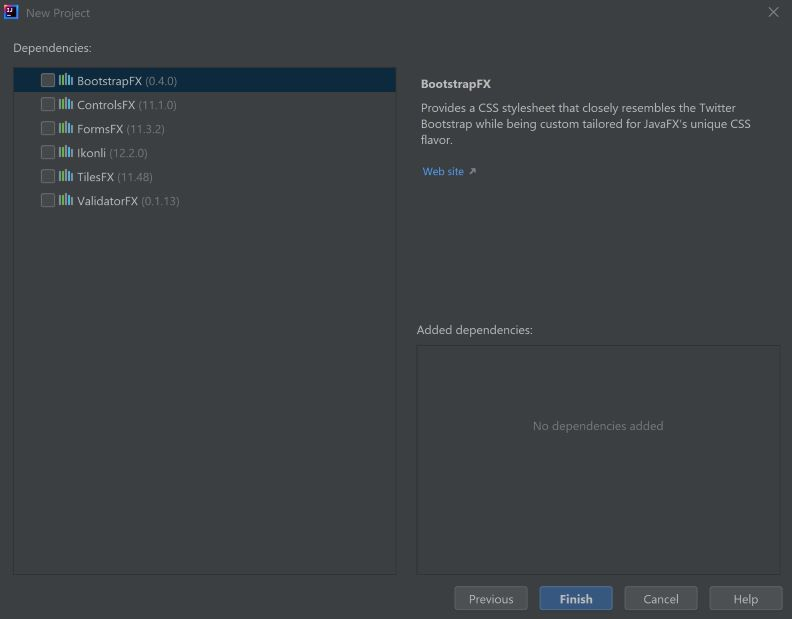
\includegraphics{DevGuideNewProject2}
    \end{center}
  \item Pull the code down from our GitHub and replace your new project's 'src' folder with the one from our GitHub
  \item Download the jSerialComm library (in .jar format) \href{https://fazecast.github.io/jSerialComm/}{here.}
  \item Open the 'File' menu and select 'Project Structure.'
    \begin{center}
    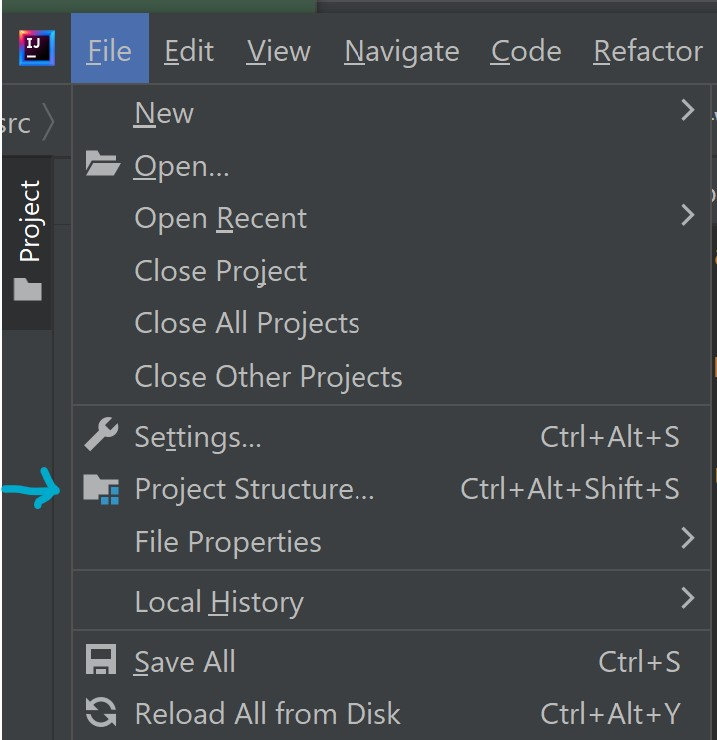
\includegraphics{DevGuideProjectStructure}
    \end{center}
\newpage
  \item Select 'Modules' under 'Project Settings', then go to the 'Dependencies' tab
    \begin{center}
    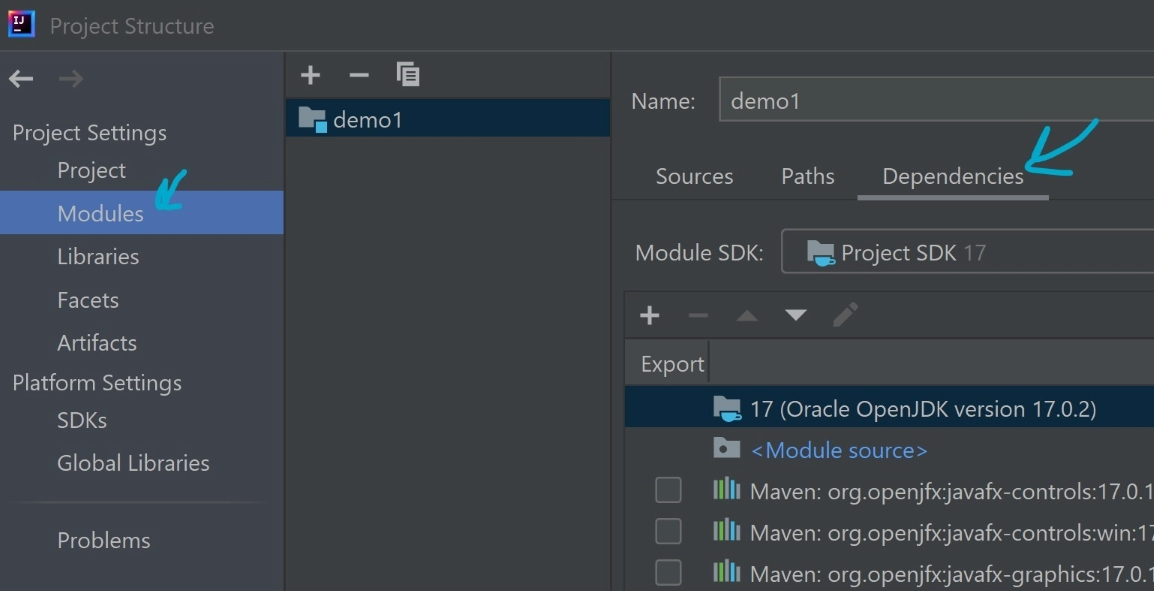
\includegraphics{DevGuideModulesDependencies}
    \end{center}
  \item Hit the '+' button, open the 'Library...' sub-menu, then select 'Java'. Use the explorer to find and select the jSerialComm<version>.jar you downloaded.
    \begin{center}
    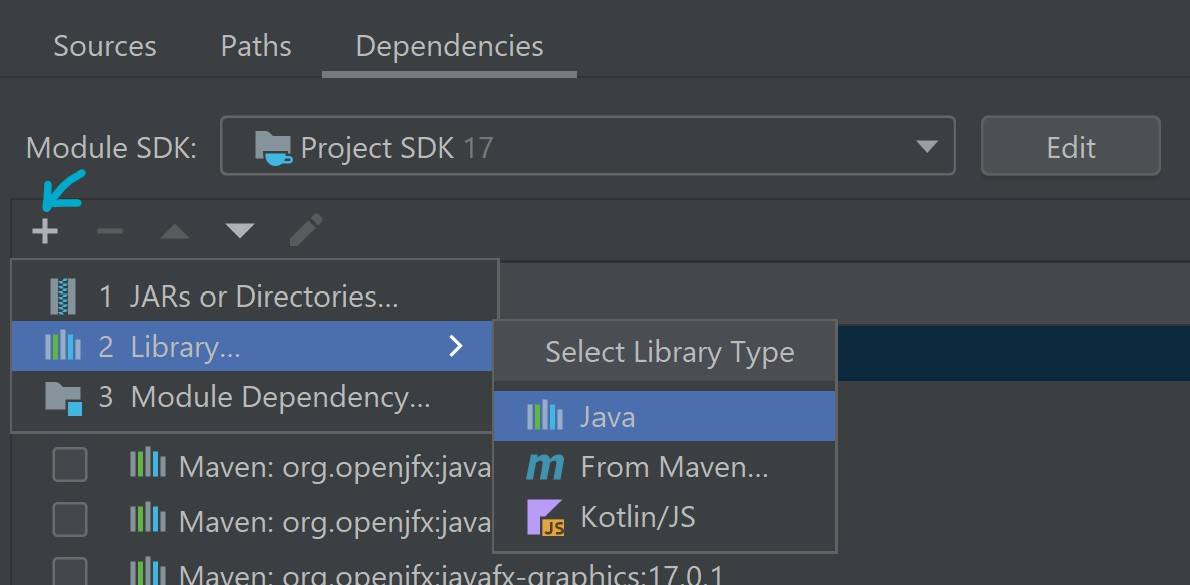
\includegraphics{DevGuideLibrary}
    \end{center}
  \item Close the 'Project Structure' window, and hit the 'Add Configuration' button in the top right of the development window
    \begin{center}
    
\includegraphics{DevGuideAddConfig}
    \end{center}
  \item Hit the '+' button, and select 'Application' in the drop down menu
    \begin{center}
    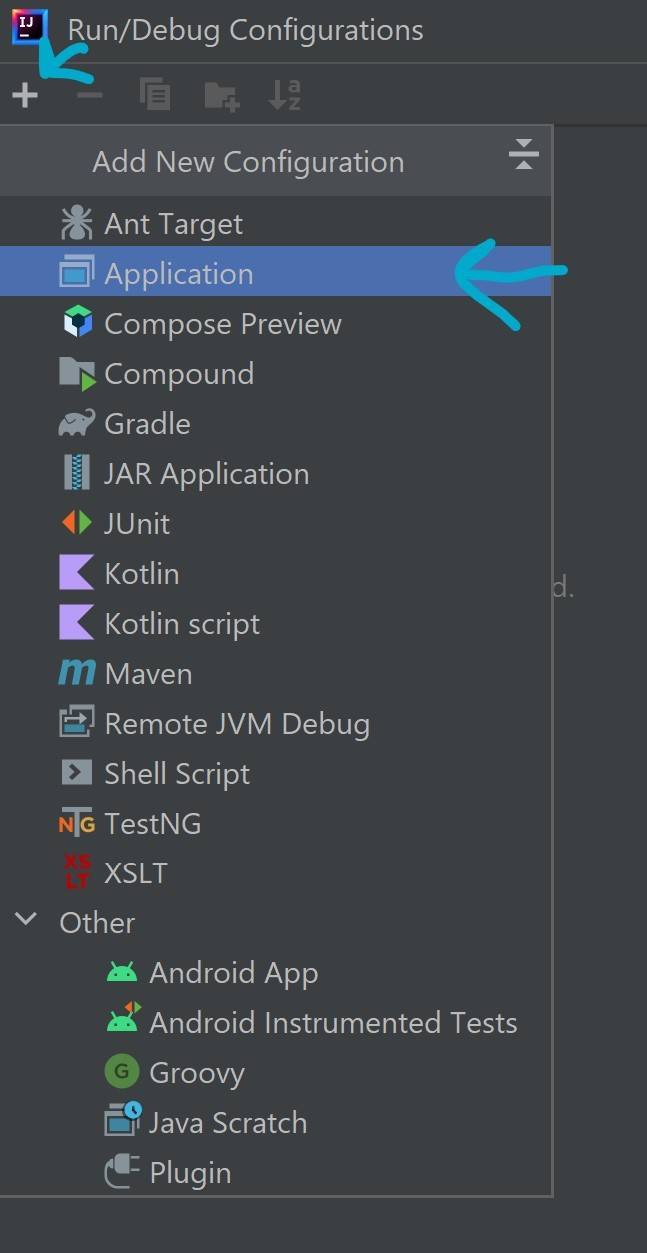
\includegraphics{DevGuideNewApplication}
    \end{center}
\newpage
  \item Give it a name (we chose 'Main'), then hit the 'File' icon in the 'Main class' text field
    \begin{center}
    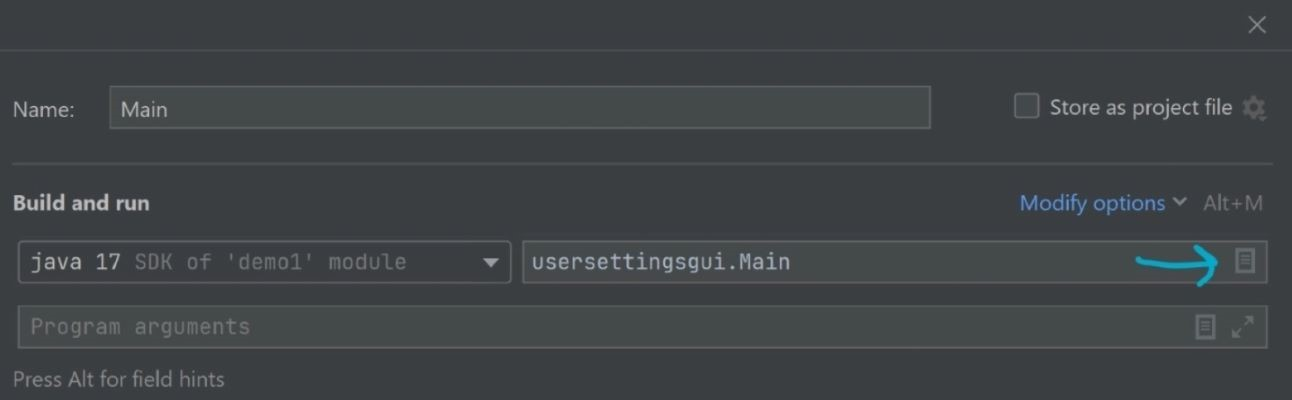
\includegraphics{DevGuideApplicationSettings}
    \end{center}
  \item Select the 'Main' class then hit 'Okay', and hit 'Okay' again in the 'Run/Debug Configurations' Window.
    \begin{center}
    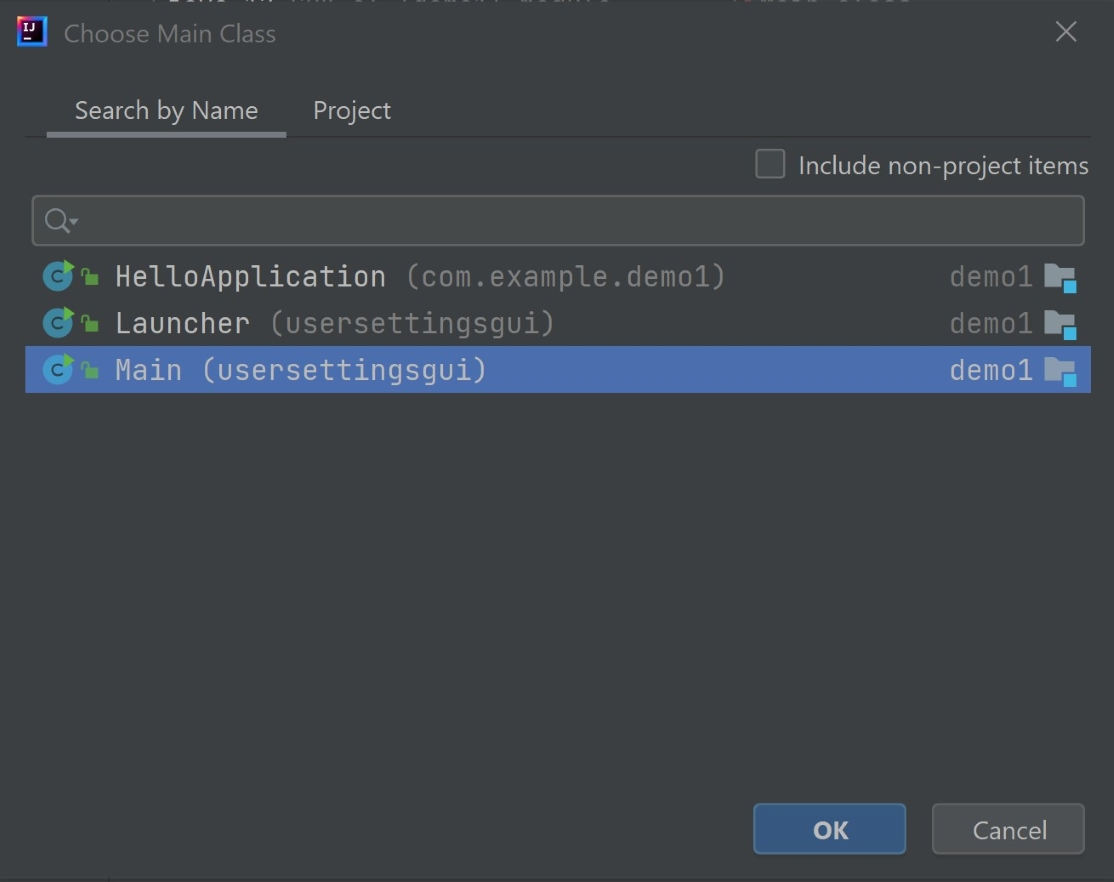
\includegraphics{DevGuideSelectMain}
    \end{center}
\newpage
  \item You can now hit the "Play" button next to where the Add Configuration button was, and the project will be built and run from IntelliJ
    \begin{center}
    
\includegraphics{DevGuideRun}
    \end{center}
\end{enumerate}

\noindent The author of this guide also found some helpful videos about IntelliJ on \href{https://www.youtube.com/@Ken-oh5yh}{Ken-oh5yh's YouTube} channel.

\end{document}